\documentclass{article}
\usepackage[utf8]{inputenc}

\usepackage{amssymb}
\usepackage{amsmath}
\usepackage{float}
\usepackage[toc,page]{appendix}
\usepackage{listings}
\usepackage{geometry}
\geometry{
a4paper,
top=1in
}

\DeclareMathOperator{\Var}{Var}
\DeclareMathOperator{\Corr}{Corr}
\DeclareMathOperator{\Cov}{Cov}

\title{Time Series Project 2}
\author{Stefan Eng and Franz Hartleitner}
\date{May 2019}

\usepackage{natbib}
\usepackage{graphicx}

\begin{document}

\maketitle

\section{Introduction}

\begin{figure}[H]
  \centering
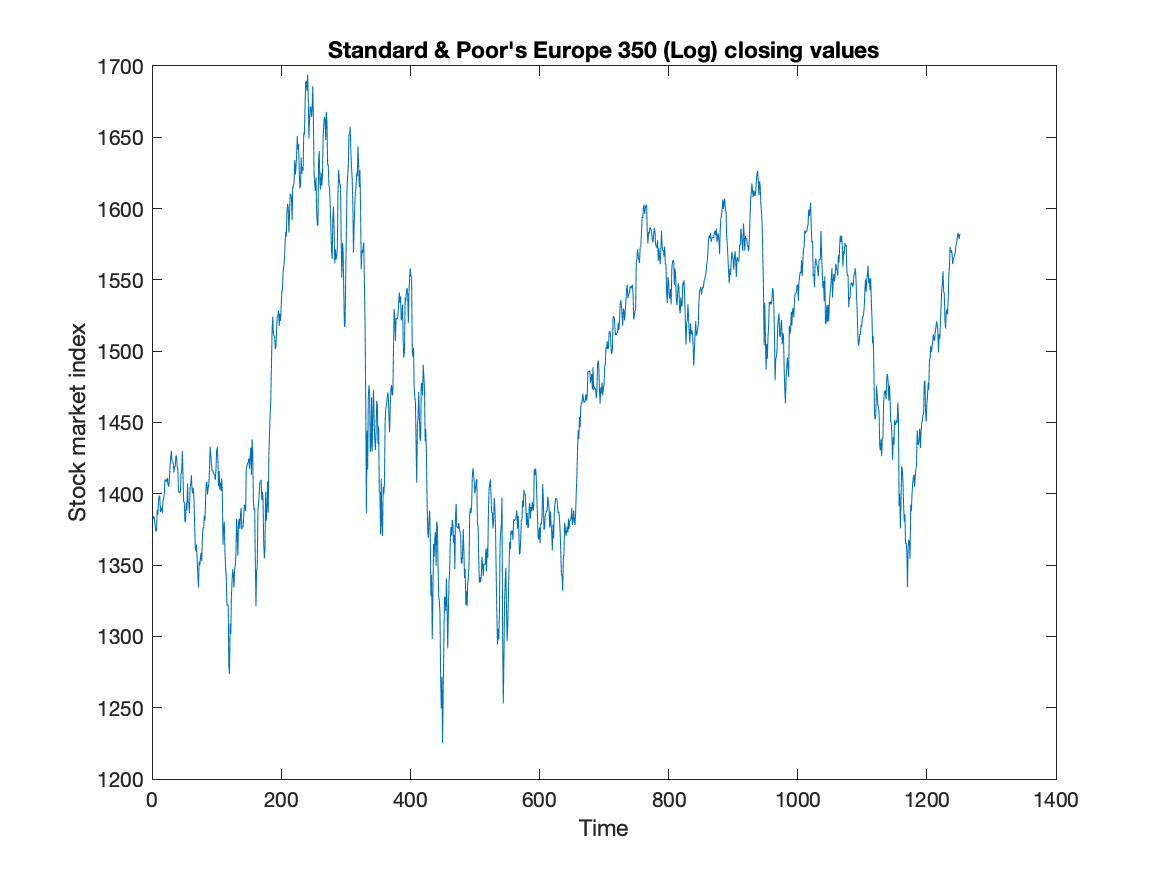
\includegraphics[width=10cm]{plots/log_index.png}
\centering
\caption{Stock market index values from April 29, 2014 to April 29, 2019}
\label{fig:log_index}
\end{figure}

In this assignment we compare GARCH models with normal and Student's t distribution.
Later, we looked into an alternative model (GJR model), which we show performs better according to BIC.


\section*{Problem 1}

\begin{figure}[H]
  \centering
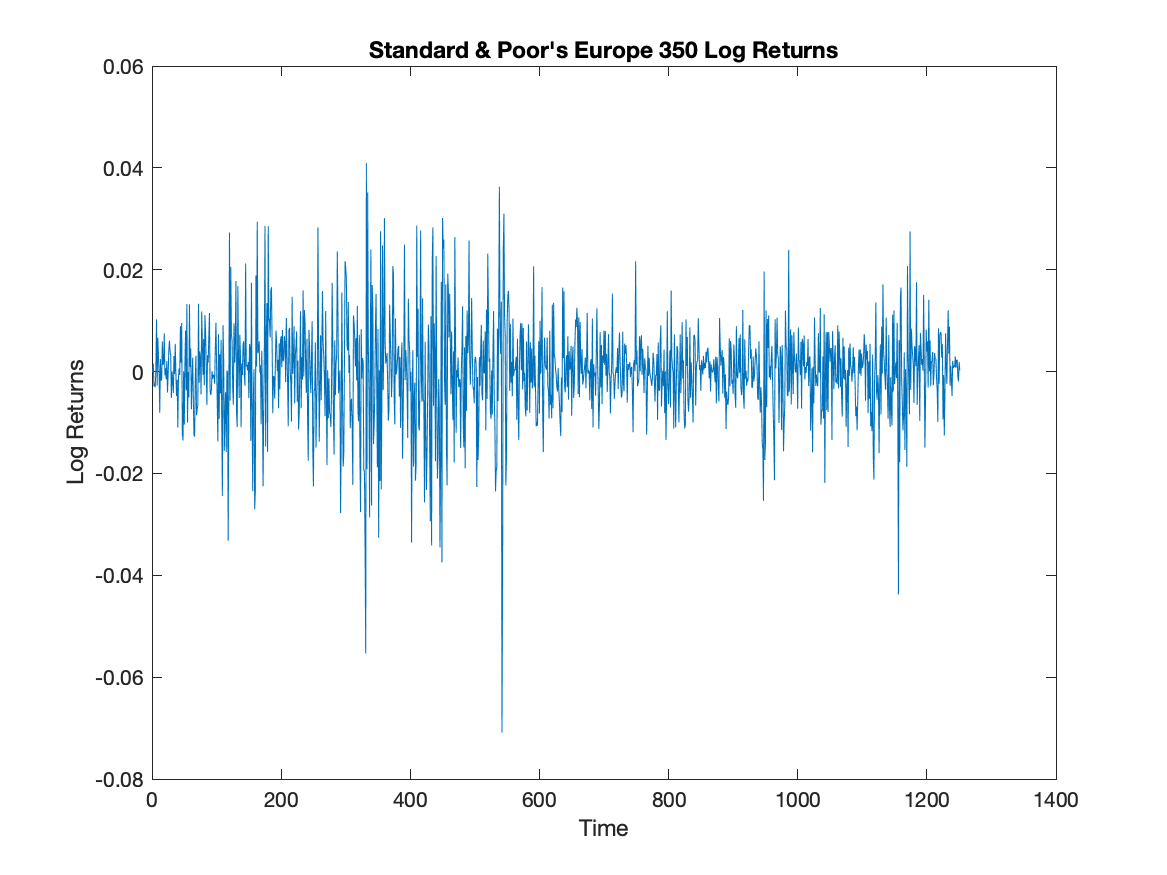
\includegraphics[width=10cm]{plots/returns.png}
\centering
\caption{Log returns from April 29, 2014 to April 29, 2019}
\label{fig:returns}
\end{figure}

We computed the log returns $X_t = \log(P_t) - \log(P_{t - 1})$ for $t = 2,\ldots, 1252$ and mean corrected the series.
In Figure \ref{fig:acf_log_rtns} we plot the autocorrelation function (ACF) for $h = 1,\ldots, 20$.
The bounds drawn on the plot correspond to $\pm 1.96/\sqrt{n}$, which we would expect 95\% of the ACF values to fall into if the returns were white noise.
For the ACF and PACF values, 90\% of the value were within the bounds $\pm 1.96/\sqrt{n}$ which is fairly consistent with white noise.
To be more precise, we use the Ljung-Box test which tests:
\begin{align*}
H_0&: X \sim IID(\mu, \sigma^2)\\
H_a& X \not \sim IID(\mu, \sigma^2)
\end{align*}
Using Matlab's Ljung-Box test \textit{lbqtest} with a lag $h = 20$, we got a p-value of 0.1331.
We fail to reject the null hypothesis at the $\alpha = 0.05$ significance level and conclude that the data is consistent with being $iid$.

In Figure \ref{fig:acf_square_rtns} we plot the ACF of the squared returns.
Why is this important to look at?
Since we have mean corrected our series, then we have that
$$
\Var(X_t) = E[X_t^2] - E[X_t]^2 = E[X_t^2]
$$
Since white noise has a constant variance, we would expect the ACF of the squared returns to not show any pattern and have most of the values within the bounds $\pm 1.96/\sqrt{n}$.
Looking at the plot, we see that there is a clear autocorrelation.
In particular, because the ACF values go up and down it sugguests that we have a non-constant conditional variance.
Thus, it is a good idea to try a GARCH model for the log returns.

\begin{figure}[H]
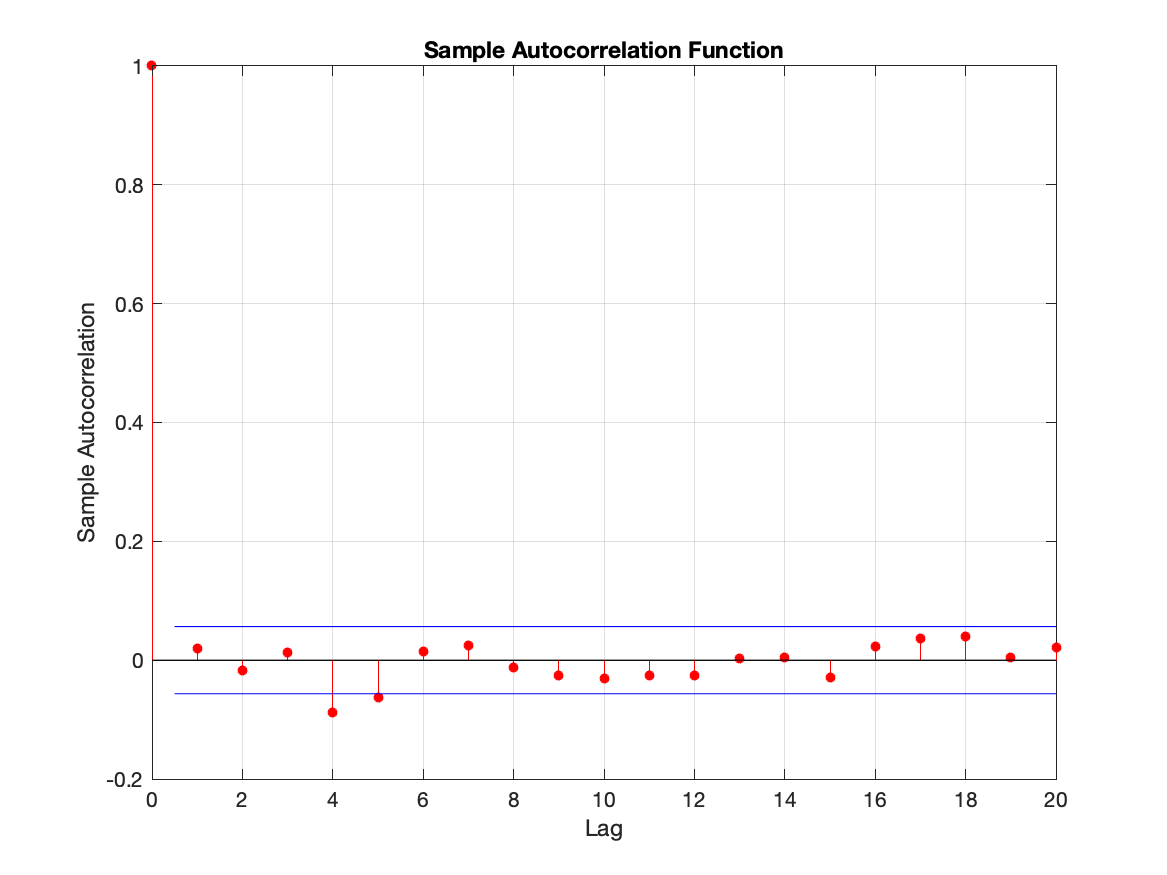
\includegraphics[width=10cm]{plots/acf_log_rtns.png}
\centering
\caption{Autocorrelation function for the log returns}
\label{fig:acf_log_rtns}
\end{figure}

\begin{figure}[H]
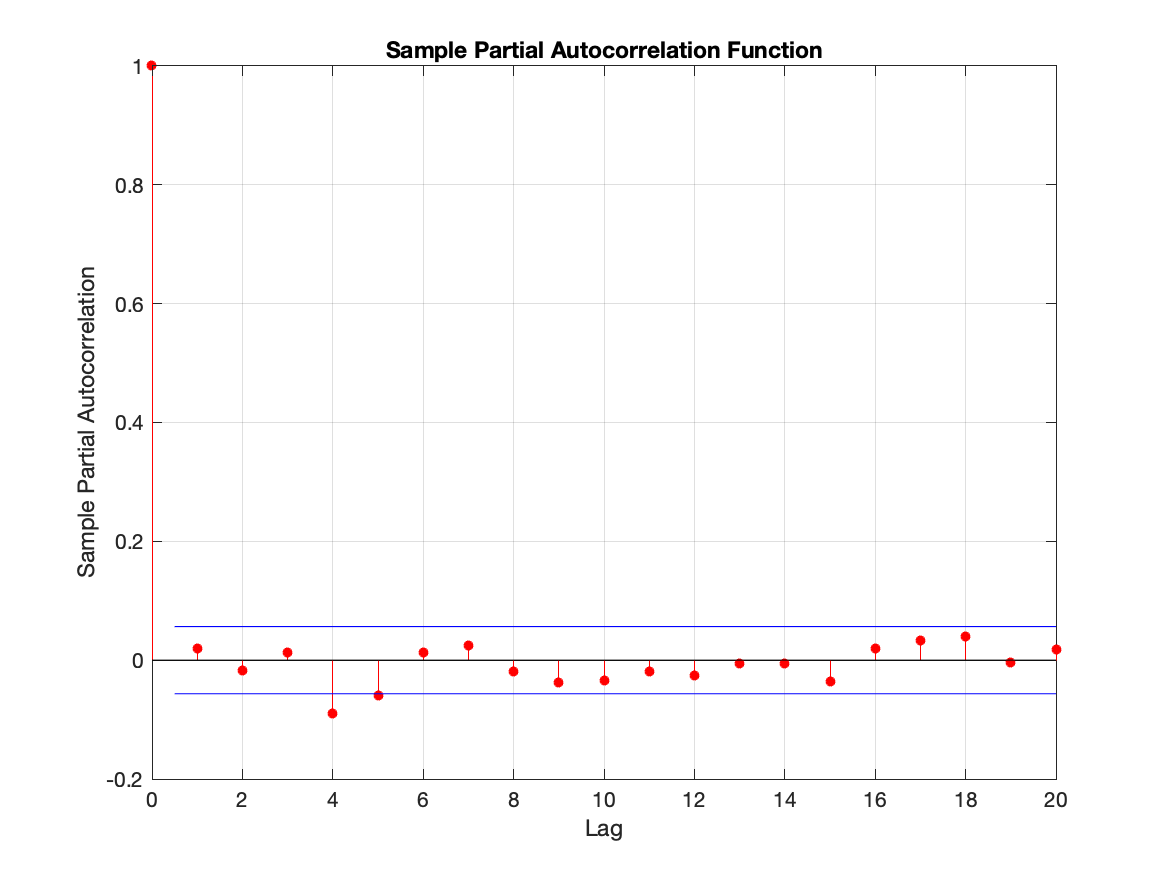
\includegraphics[width=10cm]{plots/pacf_log_rtns.png}
\centering
\caption{Partial autocorrelation function for the log returns}
\label{fig:pacf_log_rtns}
\end{figure}

\begin{figure}[H]
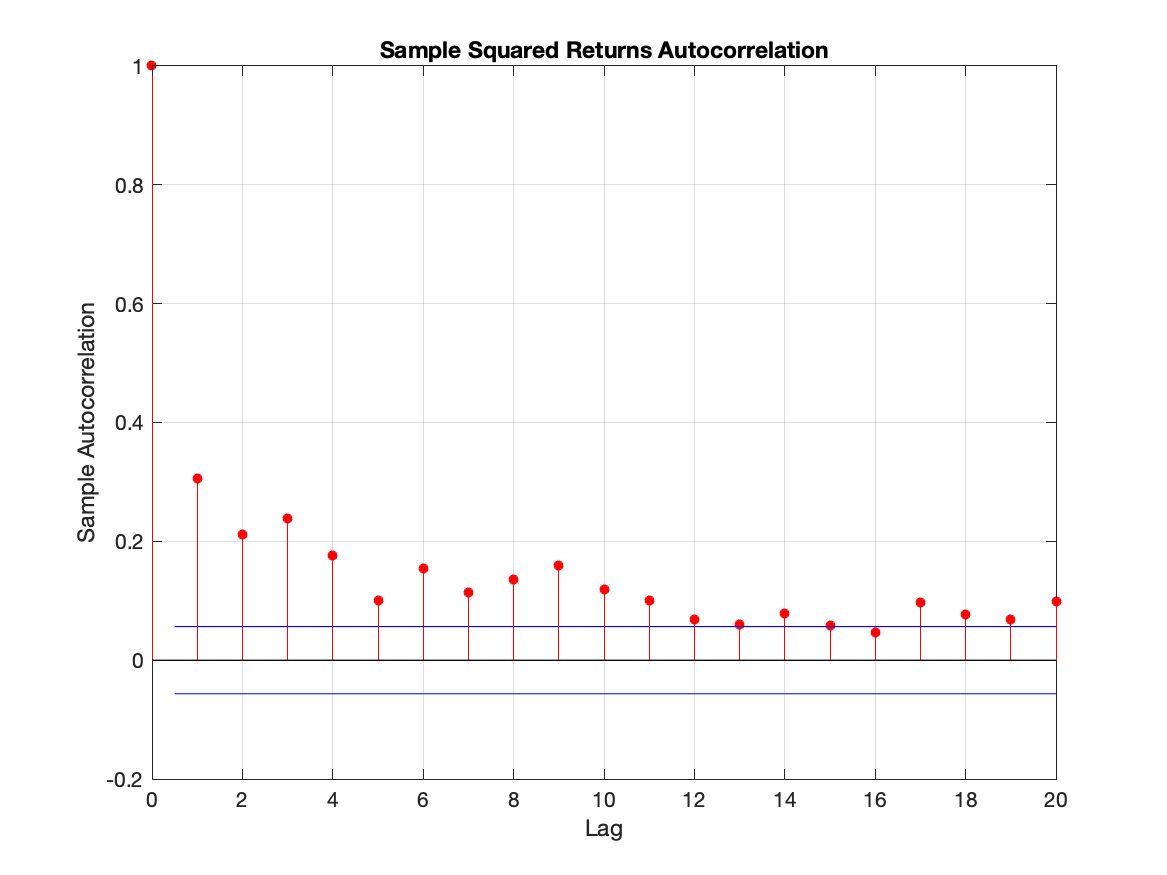
\includegraphics[width=10cm]{plots/acf_square_rtns.png}
\centering
\caption{Autocorrelation function for the squared log returns}
\label{fig:acf_square_rtns}
\end{figure}

\section*{Problem 2}

We split the data into a training set with the first 1000 values and a test set with the remaining data (251 values).
We fit a GARCH(p,q) model with Gaussian errors for each $p = 1, \ldots, 10$ and $q = 1, \ldots, 10$, resulting in 100 different models.
For each of these models we computed the BIC (Bayesian information criteria) and plotted the result in the heatmap shown in Figure \ref{fig:bic_heatmap_norm}.
The minimum model was the GARCH(1,1) model
\begin{align*}
X_t &= \sigma_t Z_t && Z_t \sim IIDN(0, 1)\\
\sigma_t^2 &= \alpha_0 + \alpha_1 X_{t - 1}^2 + \beta_1 \sigma_{t - 1}^2
\end{align*}

\begin{figure}[H]
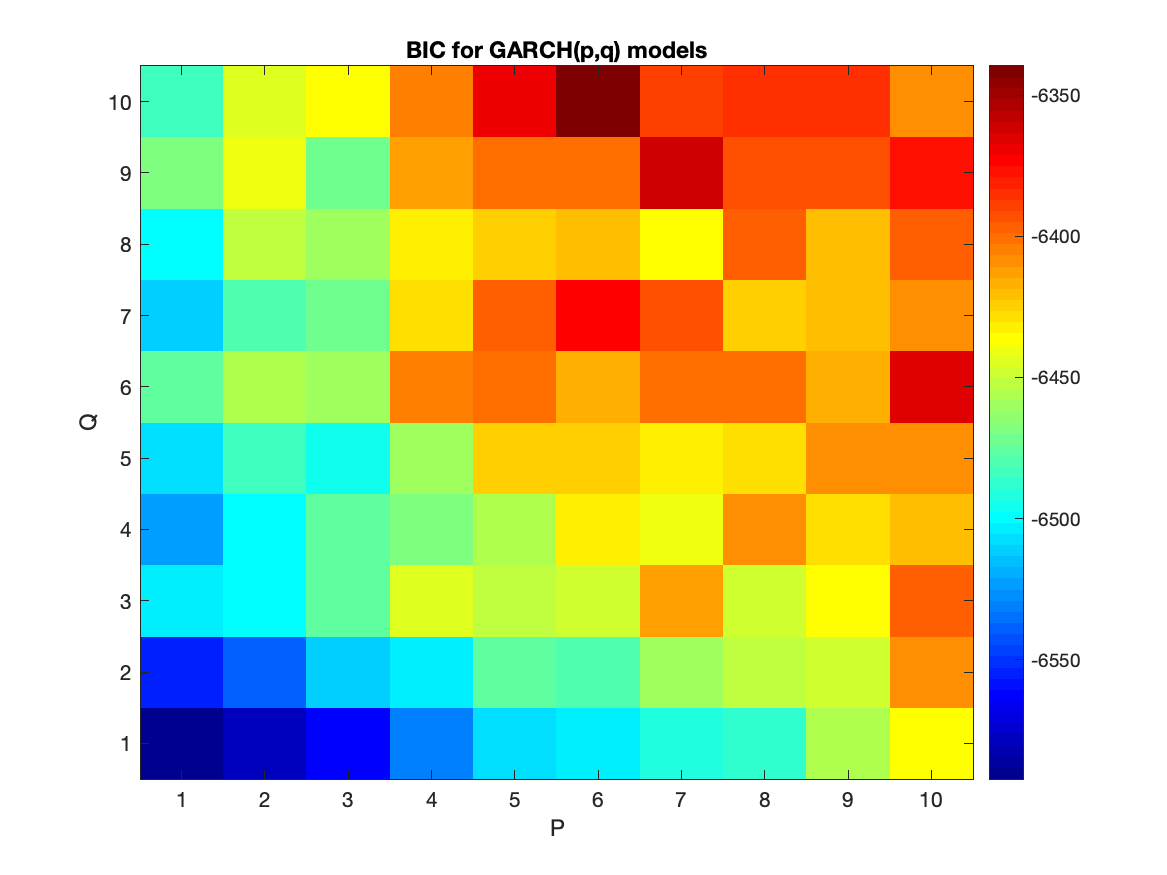
\includegraphics[width=10cm]{plots/bic_heatmap_norm.png}
\centering
\caption{BIC Heatmap for GARCH(p,q) process with Gaussian noise}
\label{fig:bic_heatmap_norm}
\end{figure}

\section*{Problem 3}

Using the GARCH(1,1) model, we computed the residuals:
$$
\hat{R}_t = (X_t - \hat{X_t})/\sqrt{\hat{\sigma_t}}
$$
for a GARCH process, $\hat{X}_t = 0$ for all $t \in \mathbb Z$.
We then plotted the residuals (Figure \ref{fig:residual_plots_norm}), QQ plot of the residuals versus standard normal, autocorrelation of residuals, and the autocorrelation of the squared residuals.
The residuals were computed by infering $\hat{\sigma_t}^2$, then dividing the training data by the square root of the infered values, $\hat{\sigma_t}$.
We would expect that if the residuals are iid random variables, then the autocorrelations $\hat{\rho}(h), 1,2,\ldots$ for sufficiently large $n$ will be approximately iid and have a normal distribution with $n^{-1}$ variance (from the lecture notes).
Thus, 95\% of the values should fall into the bounds $\pm 1.96 / \sqrt{n}$ which is draw on the ACF plots.

We can see that in the QQ plot there is some deviation from the standard normal.
We have heavier tails than we would expect with a standard normal.
The autocorrelation of the sample ACF has almost all of the values within $\pm 1.96 / \sqrt{n}$.
Similarly, the residuals squared also appear to be iid normal as all of the acf values are within $\pm 1.96 / \sqrt{n}$.
Based on the QQ-plot, it makes sense to investigate whether a Student's t distribution, which allows for heavier tails, would fit the data better.

\begin{figure}[H]
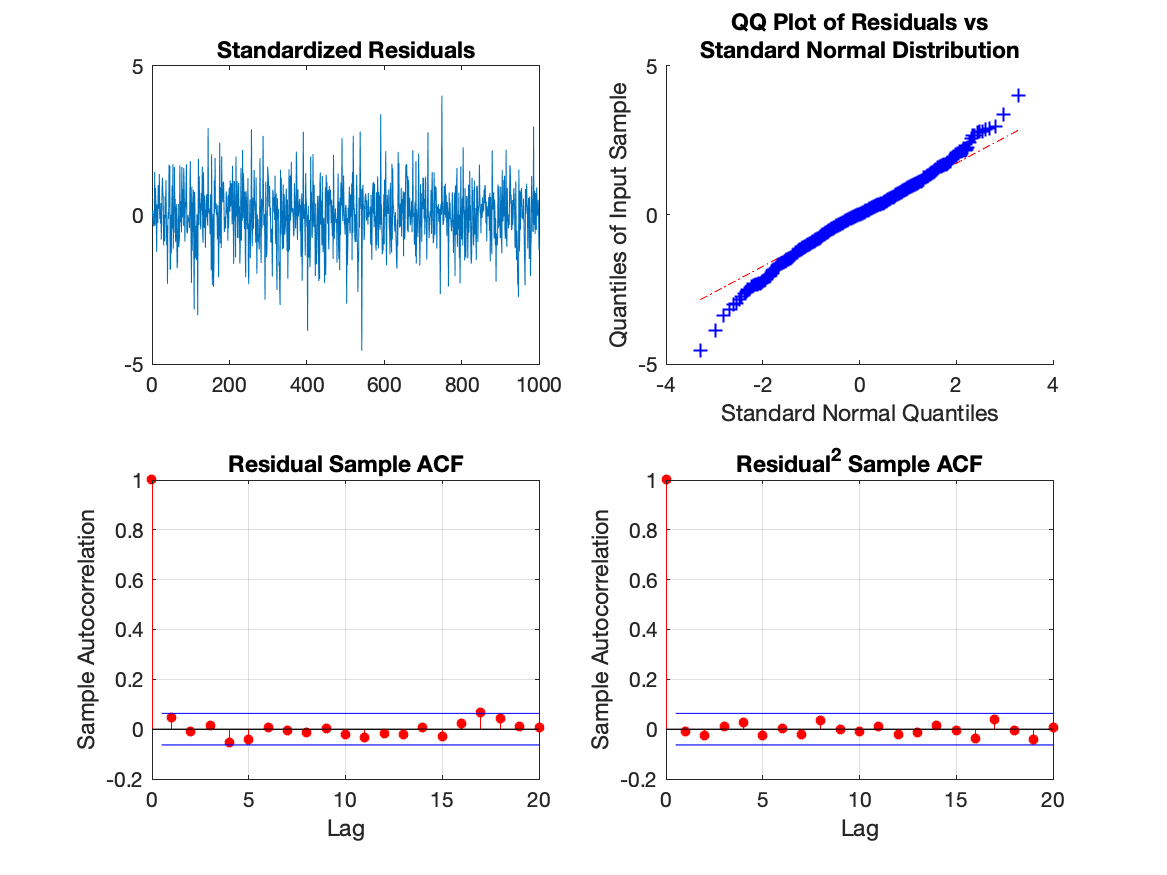
\includegraphics[width=16cm]{plots/residual_plots_norm.png}
\centering
\caption{Residual Plots for GARCH(1,1) process with Gaussian noise}
\label{fig:residual_plots_norm}
\end{figure}

\section*{Problem 4}

Now we have the model

\begin{align*}
X_t &= \sigma_t Z_t && Z_t \sim IIDt(0, 1)\\
\sigma_t^2 &= \alpha_0 + \alpha_1 X_{t - 1}^2 + \beta_1 \sigma_{t - 1}^2
\end{align*}

Where $IIDt(0,1)$ is indepedent and identically distributed Student's t distribution with some degrees of freedom $\nu$.
Again we find that the GARCH(1,1) model has the minimum BIC.
The ACF of the residuals and square residuals are consistent with iid noise as in the previous problem.
A big difference is the QQ plot which now fits almost exactly.
The model was estimated with degrees of freedom equal to 8.03.

\begin{figure}[H]
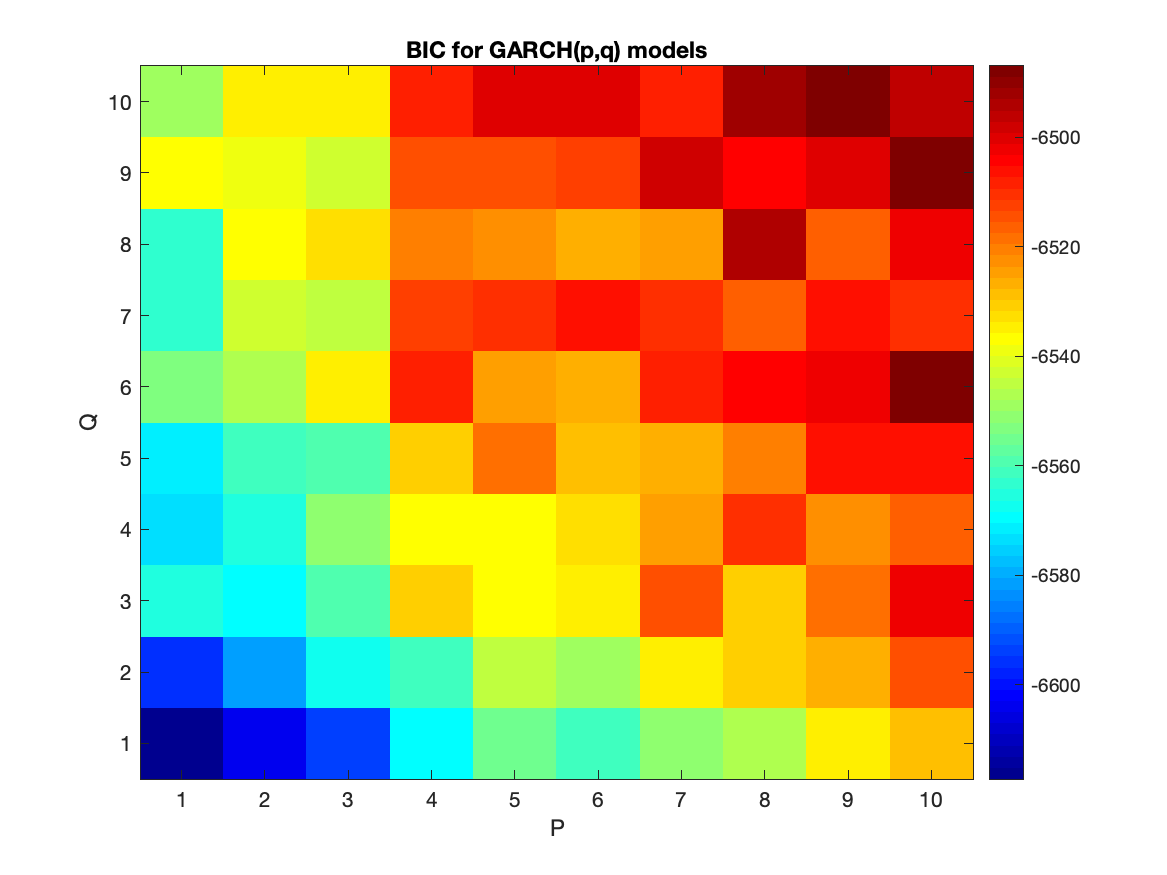
\includegraphics[width=10cm]{plots/bic_heatmap_t.png}
\centering
\caption{BIC Heatmap for GARCH(p,q) process with Student's t distribution noise}
\label{fig:bic_heatmap_t}
\end{figure}

\begin{figure}[H]
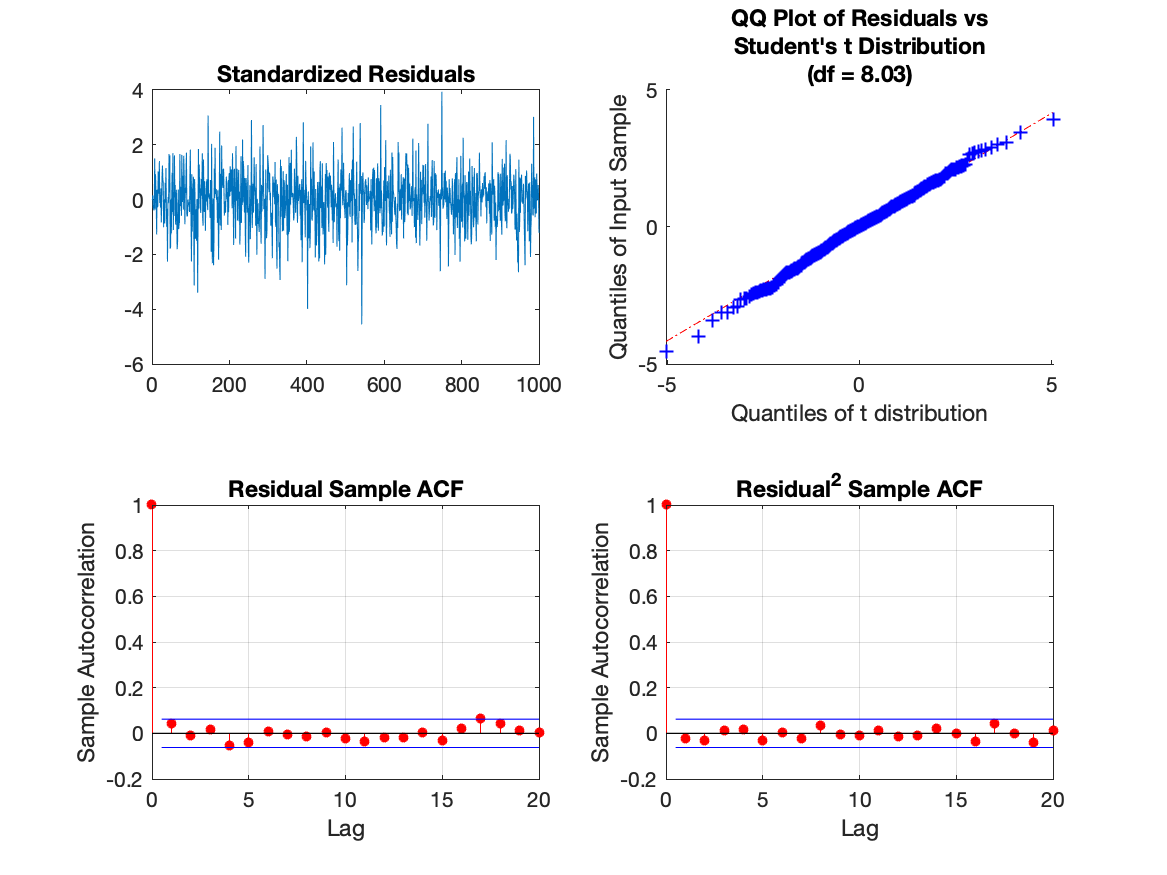
\includegraphics[width=16cm]{plots/residual_plots_t.png}
\centering
\caption{Residual Plots for GARCH(1,1) process with Student's t distribution noise}
\label{fig:residual_plots_t}
\end{figure}

\section*{Problem 5}
The distribution of $X_{t + 1}$ is $N(0, \sigma_{t+1}^2)$ when the model has normal error,
and the distribution is a student's t distribution $t(0, \sigma_{t + 1}^2)$,
where we estimate $\sigma_{t + 1}$ using
$$
\hat{\sigma}_{t + 1} = \hat{\alpha}_0 + \hat{\alpha}_1 X_t^2 + \hat{\beta}_1 \hat{\sigma}_t^2
$$
This results in confidences intervals
\begin{align*}
&\pm z_{\alpha/2} \cdot \sigma_{t + 1}\\
&\pm t_{\alpha/2, \nu} \cdot \sigma_{t + 1}
\end{align*}
Since we have $\mu = 0$ for $X_{t + 1}$.

We computed the confidence intervals for each $t = 1001,\ldots, 1251$ for both the normal model as well as the t distribution model.
At each step, we used the \textit{forecast} function in matlab and supplied all of the previous values in the log returns $X_t = \log(P_t) - \log(P_{t - 1})$ as the presample innovations.
Also, we computed the simple model which was just the sample variance of the the previous time steps, $X_1, \ldots, X_t$.

We can see in Table \ref{tab:ci_counts} that in our sample, almost all the other points fell into each of the confidence intervals (larger than 95 percent).
The plot of the confidence intervals with the points shows us that the bounds are tightest for the normal model, then the t-model and finally the sample variance model.

\begin{table}[H]
  \centering
\begin{tabular}{l | lll}
& Normal & T & Simple\\ \hline
counts & 250  & 250 & 246 \\
percentage & 0.996 & 0.996 & 0.98   \\
\end{tabular}

\caption{Count of number of time $X_{t+1}$ falls into confidence intervals}
\label{tab:ci_counts}
\end{table}

\begin{figure}[H]
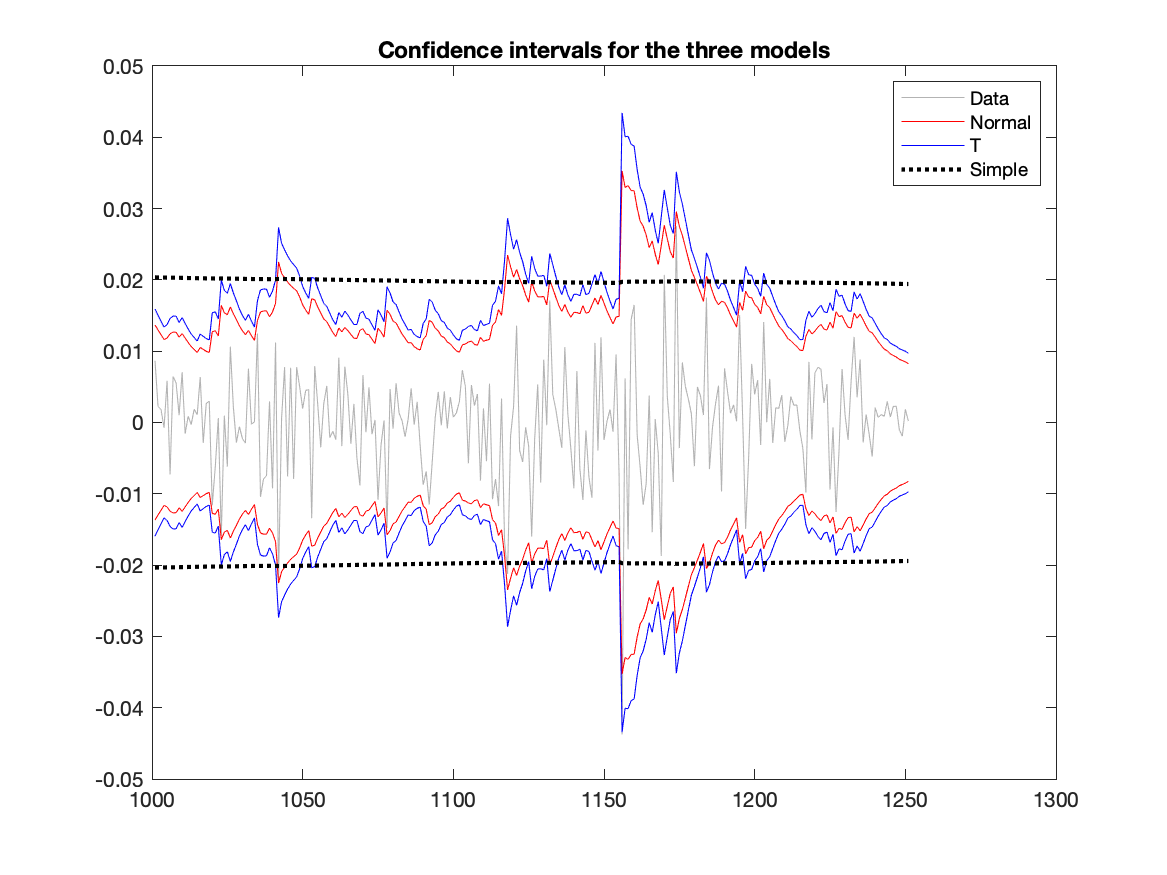
\includegraphics[width=16cm]{plots/conf_ints_overlay.png}
\centering
\caption{Confidence intervals (overlayed) for the three models}
\label{fig:conf_intervals}
\end{figure}

\section*{GJR Model}

\begin{table}[H]
  \centering
\begin{tabular}{l | l l l l}
& Normal & T & GJR(1,1) & GJR(5,3)\\ \hline
BIC & -6592.3 & -6617.3 & -6632.8 & -6635.3 \\
\end{tabular}
\caption{BIC of GARCH(1,1) Normal/T, and GJR models}
\label{tab:bic_compare}
\end{table}

We used a GJR (Glosten, Jagannathan, and Runkle) \cite{gjr1993} model which uses the same model as the GARCH(p,q) model, but includes parameters to model leverage.
$$
X_t = \sigma_t Z_t
$$
where
$$
\sigma_t^2 = \alpha_0 + \sum_{j = 1}^p \alpha_j X_{t - j}^2 + \sum_{i = 1}^q \beta_i \sigma_{t - i}^2 + \sum_{j = 1}^q \xi_j I [X_{t - j} < 0] \sigma_{t - j}^2
$$

What this allows is for us to model the volatility differently if we have a negative value (negative shock) rather than a positive value (positive shock).
We fit models for $p = 1,\ldots, 10$ and $q = 1,\ldots 10$. The minimum value model (based on BIC) was $P = 5$ and $Q = 3$ which had a BIC of $-6635.303$.
To compare the models more directly, we also looked at the GJR(1,1) model, which had a lower BIC than both of the GARCH models.
We found this to be more directly comparable to the other GARCH(1,1) models.
The results for the parameter estimates of GJR(1,1) are shown in Table \ref{tab:gjr_summary}.
A notable value is that the leverage parameter is higher than 0, which means that the negative differences in the returns will increase the conditional variance more than positive differences \cite{leverage2017}.
This does seem to match the original plot in Figure \ref{fig:returns}.

\begin{table}[H]
  \centering
\begin{tabular}{l | l l l l}
  & Value & StandardError  &  TStatistic  &    PValue                      \\
  \hline
Constant & 1.9808e-06   &   8.351e-07    &     2.372    &    0.017693   \\
GARCH\{1\}    &      0.85556   &    0.017223   &     49.676    &           0 \\
ARCH\{1\}    &      0.010588   &    0.013643   &    0.77608   &       0.4377 \\
Leverage\{1\}   &    \textbf{0.25399}   &    0.037509   &     6.7714  &    1.2755e-11
\end{tabular}
\caption{Summary of GJR(1,1) model}
\label{tab:gjr_summary}
\end{table}

\begin{appendices}

\subsection{project2.m}
\lstinputlisting[language=Octave]{project2.m}

\end{appendices}

\bibliographystyle{plain}
\bibliography{references}
\end{document}
